\begin{figure}
    \centering
    \begin{small}
    \begin{sc}
    \begin{tikzpicture}[node distance=0cm, auto]
    
    \tikzstyle{header} = [text centered]
    \tikzstyle{pict} = [inner sep=4px]
    \tikzstyle{arrow} = [thick,->,-{Latex[scale=1]}]
    

    \node [pict, label={[align=center]above:\\$0.5$}, label={[align=left]left:Grid density}] (scale1) {\includesvg[width=1.5cm]{figures/elasticities/grid/gridx0.5.svg}};
    \node [pict, right=of scale1, label={[align=center]above:Scale\\$1$}] (scale2) {\includesvg[width=1.5cm]{figures/elasticities/grid/gridx1.svg}};
    \node [pict, right=of scale2, label={[align=center]above:\\$1.33$}] (scale3) {\includesvg[width=1.5cm]{figures/elasticities/grid/gridx1.33.svg}};


    \node [pict, below=of scale1, label={[align=left]left:Grid zoom}] (zoom1) {\includesvg[width=1.5cm]{figures/elasticities/scale/zoom0.5.svg}};
    \node [pict, right=of zoom1] (zoom2) {\includesvg[width=1.5cm]{figures/elasticities/scale/zoomx1.svg}};
    \node [pict, right=of zoom2] (zoom3) {\includesvg[width=1.5cm]{figures/elasticities/scale/zoomx1.33.svg}};

    
    % \node [pict, below=of ssel, label={[align=right]left:Elastic\\sampling}] (esel) {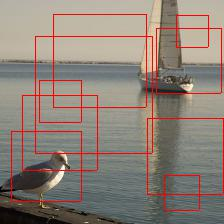
\includegraphics[width=2.5cm]{figures/teaser/3.jpg}};

    % \node [header, right] (selection) {\makecell[c]{Sampling\\selection}};
    % \node [header, right=1.4cm of selection] (patches) {\makecell[c]{Extracted\\patches}};
        
    \end{tikzpicture}
    \end{sc}
    \end{small}

    \caption{\textbf{Scale elasticities:} We use two perturbation scenarios, that change the size of a patch in a grid. The first (grid density) changes the number of patches. The second (grid zoom) keeps same number of patches but changes theirs size.}
    \label{fig:gridscalezoom}
\end{figure}